	\section{Choix de l'ordonnanceur}
	

	\subsection{Enjeux du choix de l'ordonnanceur}
	
	L'état de l'art nous a montré un vaste choix d'algorithmes qui présentent 
	des intérêts différents, et pour un certain nombre, 
	n'ayant pas encore été implémentés. \newline
	
	La première étape du travail consiste donc à départager ces algorithmes pour arrêter notre choix sur l'un d'entre eux. Ceci nécessite de clarifier nos attentes concernant le choix de l'ordonnanceur.\newline
	
	Pour rappel, les objectifs de ce travail sont de procéder à une implémentation dans 
	un \textbf{RTOS} dans plusieurs buts. 
	D'abord, en implémentant un algorithme qui n'a pas d'implémentation connue, nous 
	pouvons vérifier que ce passage de la théorie à la pratique est possible (car cela n'est pas 
	toujours évident), nous pouvons également mesurer ses performances. 
	Plus largement, nous pouvons émettre des propositions à l'attention de chercheurs 
	afin qu'ils puissent envisager de développer certains points lorsqu'ils proposent de nouveaux algorithmes. \newline
	
	Il est donc primordial de se tourner vers un algorithme qui pourra apporter sur le plan de 
	l'expérience des analyses intéressantes, c'est à dire exploitables pour la communauté. 
	Insistons peut-être sur le fait que des résultats ne sont pas nécessairement chiffrés mais 
	peuvent être des constats qualitatifs quant à la mise en œuvre elle-même.\newline
	
	\subsection{Pourquoi UEDF}
	
	Le choix le plus rationnel vis à vis des objectifs devrait se faire en fonction des 
	promesses théoriques de performance et de stabilité. 
	En effet, pour faire avancer la connaissance et permettre d'augmenter la confiance des utilisateurs 
	potentiels, il est judicieux de choisir un algorithme dont on attend au moins ceci :
	\begin{itemize}
		\setlength\itemsep{0.1em}
		\item Un algorithme global
		\item Qui minimise le nombre de migrations [\ref*{migration}]
		\item L'ordonnanceur est optimal pour la classe périodique
		\item Il n'a pas bénéficié d'une implémentation sur un \textbf{RTOS}
		\item Il promet des performances intéressantes
	\end{itemize}
	
	Le premier choix a été \hyperref[RUN]{RUN}[\ref*{RUN}], puis finalement, son descendant, \hyperref[QPS]{QPS}[\ref*{QPS}]. Ces choix étant guidés 
	sur leur intérêt d'ordonnanceurs en tant que tels.
	Toutefois, l'aspect très théorique des papiers les présentant a rendu la première phase de travail difficile. 
	En outre, nous n'avons pas trouvé d'implémentation ou de simulation malgré nos recherches.
	Finalement, nous n'avons pas réussi à entrer en contact avec les créateurs de ces algorithmes. \newline
	
	En effet, la possibilité de contacter les créateurs d'un algorithme peut singulièrement améliorer le 
	travail. Cela étant, cette nécessité découle du caractère très théorique de la littérature disponible
	et du manque fréquent de prise en considération des contraintes pratiques d'implémentation. 
	Pour illustrer cette remarque, un exemple assez commun est la non prise en considération 
	du fait que le fonctionnement des ordinateurs est évidemment discret, là où les 
	calculs présentés se basent sur un fonctionnement continu.
	Toute mise en pratique nécessite de faire des arrondis, ceux-ci doivent être cohérents.\newline
	
	Nous pouvons aussi évoquer les moments où l'algorithme doit faire des calculs. 
	Dans un modèle, on peut arrêter l'exécution quand on le veut, 
	avec des temps de surcoût négligeables. 	
	Dans la réalité, comme on le verra, cela 
	n'est pas le cas. 
	Les auteurs qui connaissent bien ce fonctionnement auront la possibilité de devancer certaines questions.
	Néanmoins, dans le cas d'un papier très théorique qui s'emploie à faire des démonstrations mathématiques, 
	cela n'apparaîtra pas forcément. \newline
	
	\textbf{UEDF} bénéficie quant à lui d'une littérature qui développe mieux l'aspect pratique, et cela a orienté notre choix.\newline
	
	En d'autres termes, l'implémentation d'un ordonnanceur peut s'avérer une tâche bien compliquée selon le degré de 
	description pratique et d'anticipation des problèmes que les auteurs auront pris la peine d'aborder 
	dans les papiers publiés.
	\newline
	
	
	Finalement, c'est un argument quant à la communication (clarté, possibilité de poser des questions) 
	qui a fixé le choix. Par conséquent, c'est \textbf{UEDF} qui a été sélectionné, car 
	non seulement il respectait 
	les promesses énoncées auparavant, mais aussi, en plus d'être très bien documenté, 
	nous pouvions poser nos questions directement à l'un de ses créateurs. Néanmoins, ses paramètres sont moins idéaux, 
	et nous avons revu nos attentes quant à l'efficacité à la baisse. Cela n'a en rien 
	modifié l'objet scientifique, à savoir le regard critique et la proposition d'améliorations 
	afin de stimuler et faciliter des implémentations futures, mais cela a sans doute 
	diminué les performances finales obtenues, tel que nous le verrons dans la partie \hyperref[resultats]{résultats} [\ref*{resultats}].\newline
	
	
	\section{Présentation UEDF}\label{contexte}
	
	Nous avons déjà présenté précédemment \textbf{UEDF}, de façon globale et succincte. 
	Dans cette partie, nous allons détailler l'algorithme afin d'en avoir une meilleure compréhension. Cela 
	permettra de mesurer la différence entre les attentes théoriques et les résultats obtenus.\newline
	
	%\todo{etat de l'art, parler de généralisation horizontale/verticale}
	
	\subsection{Définitions spécifiques}
	Dans un premier temps, nous posons quelques définitions qui sont nécessaires à la compréhension de l'algorithme. 
	Par ailleurs, par souci de clarté, nous simplifions les calculs en supposant que les offsets [\ref*{offset}] des tâches 
	sont nuls dans la partie qui suit, cela ne change pas l'algorithme mais rend les explications moins 
	complexes.
	
	\subsubsection{Tâche active}\label{tacheactive}
	Ce qui définit une tâche \og{}active\fg{} peut différer selon le contexte. Dans l'approche d'\textbf{UEDF}, une tâche est 
	considérée comme active si un travail a été relâché et que ce travail n'a pas encore atteint son échéance. 
	Un travail $\tau_i$ est actif s'il a été relâché sur ou avant $t$ et que $d_i(t) \geq t$.
	Une tâche peut donc 
	être considérée comme active même si l'exécution d'un travail en cours est terminée. 
	Concrètement, si une tâche est périodique à échéance implicite [\hyperref[echeancesurrequete]{\ref*{echeancesurrequete}}], elle est active en permanence dès le 
	premier relâchement de travail. Le travail sera actif durant son relâchement jusqu'à ce que $t \geq d_i(t)$, où 
	une nouvelle instance de la tâche $\tau_i$ sera relâchée.
	
	
	\subsubsection{Ensemble des tâches actives}\label{ensembledestachesactives}
	L'ensemble des tâches actives est écrit $A(t)$ dans les formules qui suivent. Notons que dans un système 
	périodique à échéances implicites \hyperref[echeancesurrequete]{[ \ref*{echeancesurrequete} ]}, cet ensemble 
	sera toujours composé des mêmes tâches.\newline
		
	Dans \textbf{UEDF}, on effectue le parcours d'une liste des tâches actuellement actives dans le système, 
	cette liste étant ordonnée par échéances pour les besoins de l'algorithme. 
	On notera $sorted\_ActiveList(t)$ la liste triée créée à partir de l'ensemble des tâches $A(t)$.\newline
	
	Pour décrire \textbf{UEDF}, nous allons le décomposer en étapes.
	À chaque fois qu'un nouveau travail est relâché, cela va provoquer le calcul d'$Allot_{ij} \forall i \in A(t), \forall j \in \{1 ... m\}$.

	\subsubsection{Allot}\label{allot}
	Les tâches actives [\ref*{tacheactive}] sont donc ordonnées dans la liste $sorted\_ActiveList(t)$. 
	La priorité est définie selon l'échéance, la plus petite étant la plus prioritaire, comme dans \hyperref[EDF]{EDF [\ref*{EDF}]}.
	Dans cette phase, l'algorithme va \og{}réserver\fg{} des tranches de temps d'exécution des tâches sur les 
	processeurs, cela en calculant un tableau de valeur : \newline
	$allot_{ij}$ pour $i \in \{0, nb\_de\_taches - 1\}$, pour $j \in \{0, nb\_processeurs - 1\}$.
	La valeur $allot_{ij}$ représente le nombre d'unités d'exécution de la tâche $i$ réservé sur le processeur $j$.\newline
	Si cette valeur est positive, alors le temps $allot_{ij}$ du travail $i$ est réservé sur le 
	processeur $j$. Si cette valeur est égale à $0$, aucun temps n'est réservé 
	à l'exécution de la tâche $\tau_i$ sur le processeur $\pi_j$. Cela permet la constitution d'une liste, 
	\textbf{Eligible}.\newline


	Les calculs sont longuement décrits et expliqués dans la thèse de G. Nelissen \cite{nelissen_u-edf_2012}, aussi nous invitons 
	le lecteur curieux à se référer à ce document pour de plus amples détails. Mais en résumé, 
	ce calcul se déroule de cette façon :
	
	Nous posons :
	\begin{itemize}
		\setlength\itemsep{0.1em}
		\item $delay = d_i(t) - t$
		\item $ret_i = wcet - $ le nombre d'unités de temps déjà exécutées
		\item L'opérateur $[x]_a^b \defeq \max\{a, \min\{b, x \}\}$
	\end{itemize}

	Dans l'algorithme qui suit, le but est d'\og{}allouer\fg{} le temps qui reste à exécuter pour chaque travail 
	actif aux processeurs présents.
	Pour ce faire, on calcule la valeur maximale $allot_{max}$ que l'on peut réserver sur un processeur, 
	en faisant appel à la somme de l'\textit{utilisation} des travaux déjà traités ($W$).
	Cela permet de calculer le minimum entre ce maximum et le nombre d'unités d'exécutions qui 
	restent effectivement à allouer pour le travail $\tau_i$, et finalement, de l'allouer dans 
	$allot_{ij}$.

	\label{algouedf}
	\begin{algorithm}[H]
		\caption{Compute Allot}
		\begin{algorithmic}
			\REQUIRE $sorted\_ActiveList(t)$
			\STATE $W = 0$
			
			\FORALL{ $j \leftarrow \{1 ...m\} $}
				\item $RES_j \leftarrow 0$
				\item $ALLOT_j \leftarrow 0$
			\ENDFOR
	
			\FORALL{ $\tau_i \in sorted\_ActiveList(t) $}
				\item $prev_i \leftarrow 0$
				\FORALL{ $j \leftarrow \{1 ...m\} $}
					\item $RES_j \leftarrow RES_j + \{[W]_{j-1}^{j} - (j - 1)\}\times (d_i(t) - d_{i-1}(t))$
					\item $allot_{max} \leftarrow delay - ALLOT_j - RES_j - prev_i$
					\item $allot_{ij} \leftarrow min\{allot_{max}, ret_i - prev_i\}$
					\item $prev_i \leftarrow prev_i + allot_{ij}$
					\item $ALLOT_j \leftarrow ALLOT_j + allot_{ij}$
				\ENDFOR
				\item $W \leftarrow W + U_i$
			\ENDFOR
		\end{algorithmic}
	\end{algorithm}
	
	Dans l'exemple qui suit, notre système est composé de deux tâches :
	\begin{enumerate}
		\setlength\itemsep{0.1em}
		\item $\tau_1 : \{o:0; w:30; d=p:60;\}$
		\item $\tau_2 : \{o:0; w:60; d=p:80;\}$
	\end{enumerate}
	\begin{figure}[H]
		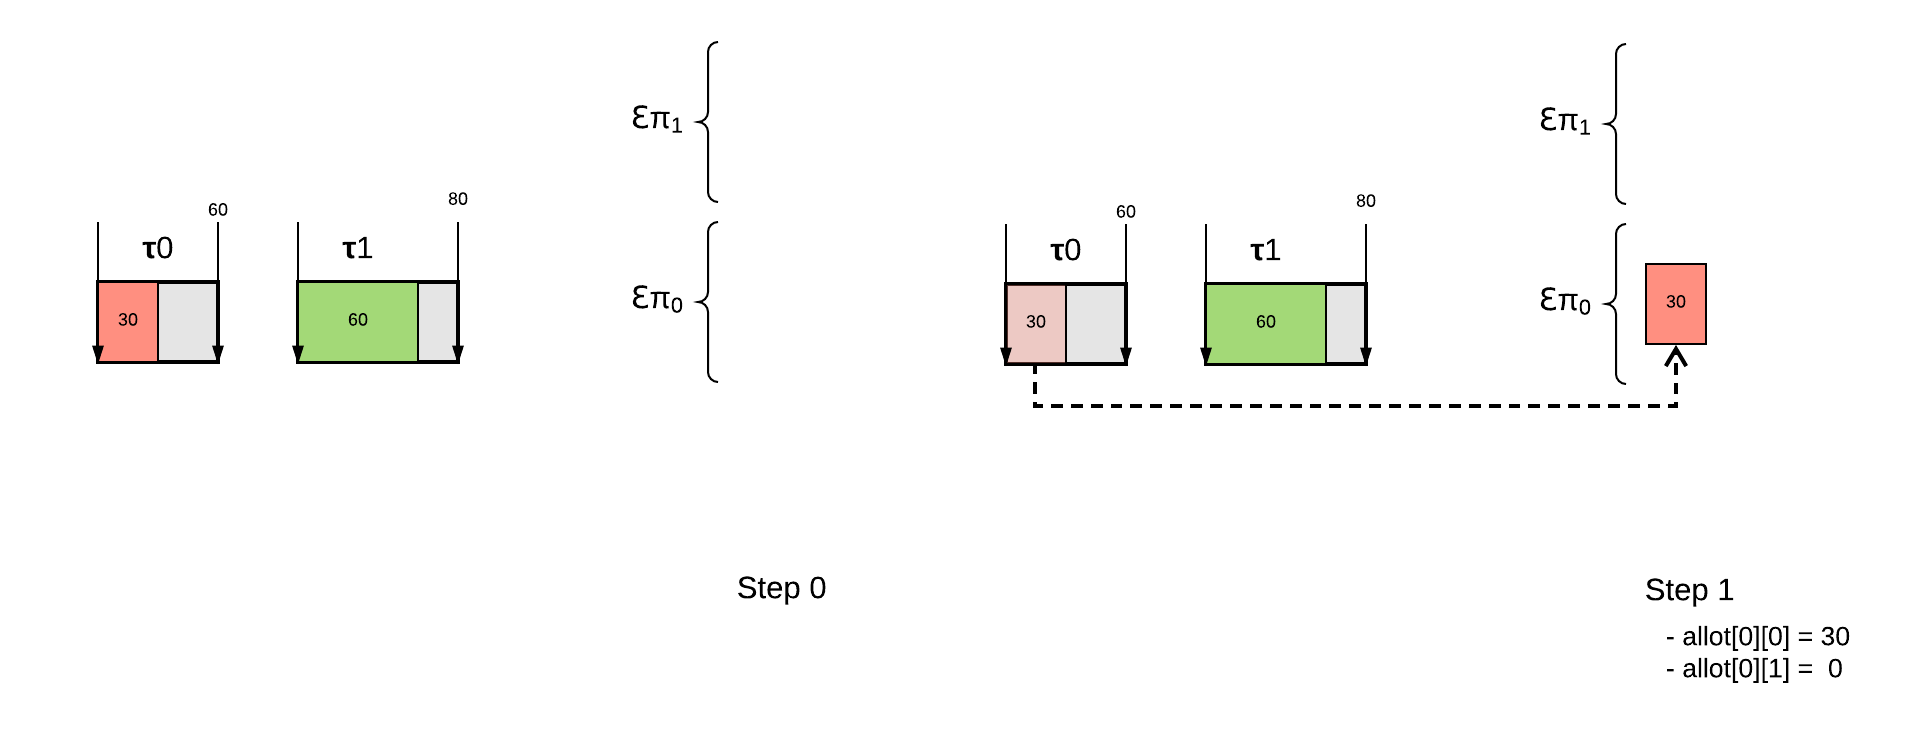
\includegraphics[scale=1]{img/uedf/uedf12}
		\caption{étapes 0 et 1}
	\end{figure}
	\begin{figure}[H]
		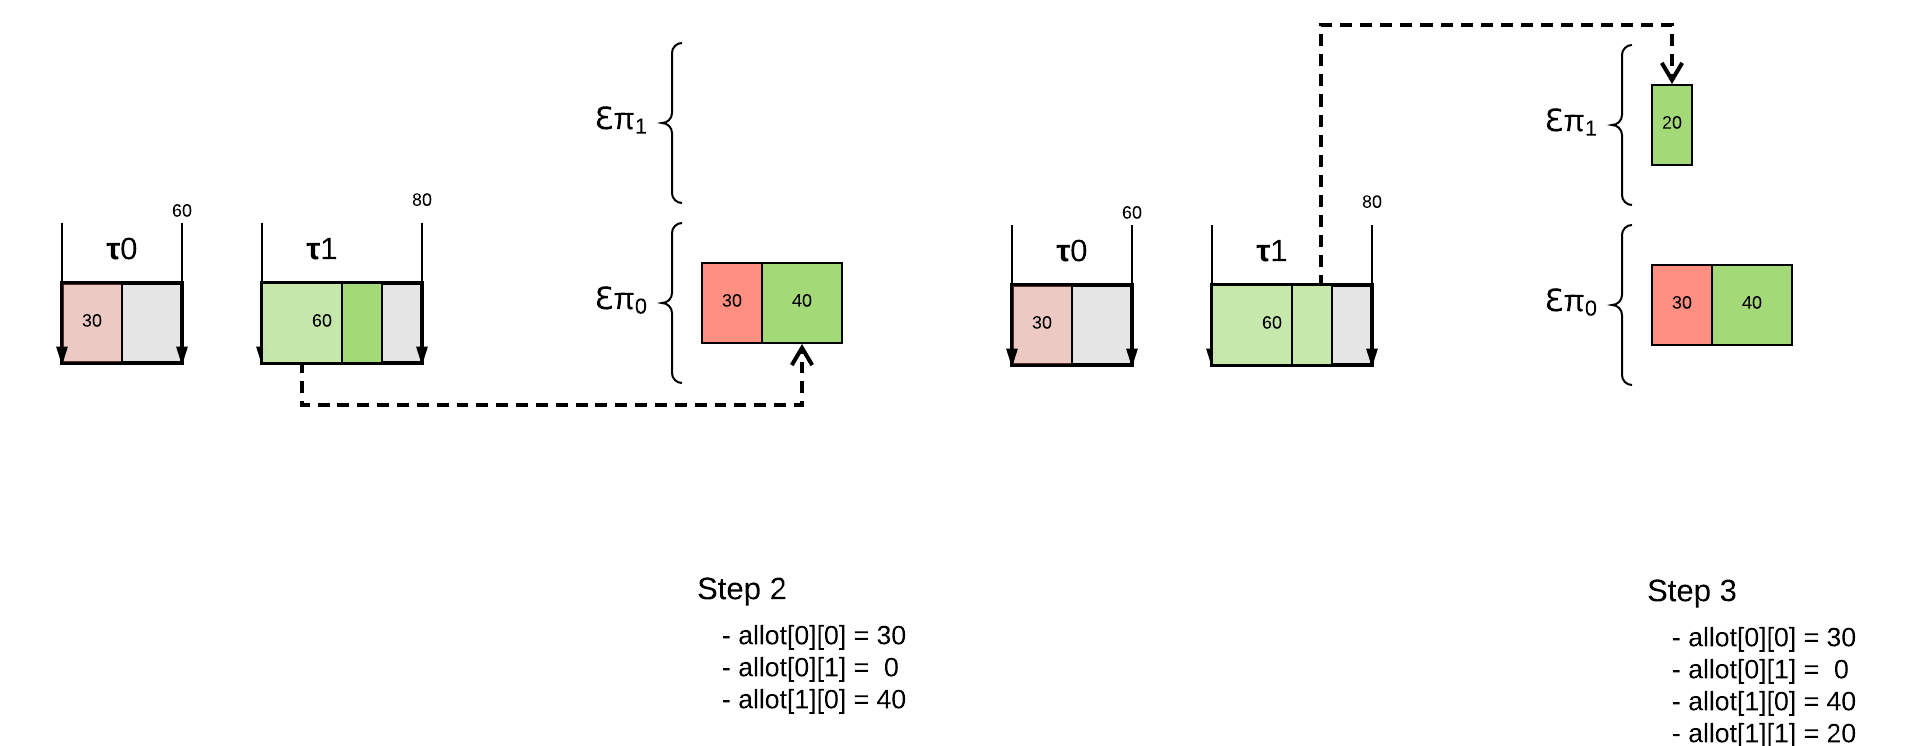
\includegraphics[scale=1]{img/uedf/uedf34}
		\caption{étapes 2 et 3}
	\end{figure}
	\subsubsection{Eligible}
	À ce stade, aucune décision d'ordonnancement n'est encore prise, mais des ensembles de tâches (\textit{Eligible}, 
	noté $\epsilon$ dans la suite) sont créés sous forme de listes. Chaque liste \textit{Eligible} définit 
	les seules tâches que les processeurs associés peuvent exécuter (en cela, cette phase d'\textbf{UEDF} peut 
	être considérée comme une phase de partitionnement) durant l'exécution à venir.\newline
	
	Notons que les calculs fournis par l'algorithme permettent en théorie de \og{}remplir\fg{} 
	la charge d'un processeur à 100\% d'utilisation avant de passer au suivant. Concrètement, 
	cela signifie que si la première tâche a une utilisation de moins de 100\%, elle sera suivie par 
	au moins une partie d'une autre.\newline
	
	Les valeurs d'$Allot$ ne doivent pas être considérées comme le temps d'exécution qui sera réellement 
	exécuté sur le processeur. Il faut garder à l'esprit qu'à chaque relâchement de travail, 
	$Allot$ sera recalculé. 

	\subsubsection{Prise de décision}
	La phase de décision de l'ordonnancement se déroule lors de la phase suivante.
	\textbf{UEDF} s'inspire pour finir de \textbf{EDF-Delay}. 
	Cet algorithme est très simple :
	\begin{itemize}
		\setlength\itemsep{0.1em}
		\item Une tâche $\tau_i \in \epsilon_j, j \in m$ est attribuée à un processeur $\pi_j$ si aucun autre processeur d'index plus bas n'est en train de l'exécuter
		\item $\tau_i$ s'exécute sur le processeur $\pi_j$ tant qu'$allot_{ij} > 0$
	\end{itemize}


	\subsubsection{Déroulement}	
	L'algorithme \hyperref[algouedf]{$Compute Allot$ [\ref*{algouedf}]} est à effectuer à chaque relâchement de tâche. La valeur $Allot_{ij}$ 
	doit être mise à jour à chaque prise de décision. Une décision est attendue pour chacun des événements suivants :
	\begin{itemize}
		\setlength\itemsep{0.1em}
		\item Une instance de tâche (travail) a été relâchée\\
		 $\sum_{i \in A(t)}\sum_{1}^{m}allot_{ij} = WCET$
		\item Le temps alloué sur un processeur a été exécuté, dans ce cas\\ $\exists i \in A(t), \exists j \in m : allot_{ij} = 0$
		\item Un travail est terminé complètement : \\
		$\sum_{i \in A(t)}\sum_{1}^{m}allot_{ij} = 0$.
	\end{itemize}
	
	On peut voir en théorie l'ordonnancement de trois tâches en annexe, afin de mieux comprendre le déroulement d'une exécution.
	À titre de remarque, le travail d'illustration d'une exécution nous semble 
	important pour procéder à une implémentation, sinon le risque est d'omettre le développement 
	d'outils indispensables au bon déroulement de l'exécution. L'algorithme n'est pas trivial à mettre en œuvre.
	\todo{gantt chart avec exemple 30;60, 60; 80, 60;80}
	\newline
	
	Nous pouvons déjà formuler ici une nuance par rapport à la théorie et les attentes que l'on peut en avoir 
	en pratique : 
	nous savons dès le départ que l'algorithme \textbf{UEDF} est assez gourmand en calcul puisque chaque relâchement de 
	tâche va provoquer l'exécution de l'algorithme $Compute Allot$, or, le calcul de cette valeur 
	implique un parcours de toutes les tâches ordonnées, pour chaque processeur. 
	Outre qu'il est nécessaire de gérer une structure de données efficace, nous pouvons 
	déjà considérer que le tri de la structure sera d'un coût non négligeable lors de l'exécution. \newline
	
	Par ailleurs, le calcul même de $Compute Allot$ implique lui aussi une certaine complexité.
	Ainsi :
	\begin{itemize}
		\setlength\itemsep{0.1em}
		\item soit $m$ le nombre de processeurs
		\item soit $n$ le nombre de tâches actives [\ref*{tacheactive}] du système
		\item $Compute Allot \in O(m\times n)$
	\end{itemize}

	Et pour finir, régulièrement, la valeur $allot_{ij} \forall i \in TaskSet, \forall j \in m$ doit être mise 
	à jour, dont la complexité est donc :
	\begin{itemize}
		\setlength\itemsep{0.1em}
			\item soit $m$ le nombre de processeurs
			\item soit $n$ le nombre de tâches actives [\ref*{tacheactive}] du système
			\item $update Allot \in O(m\times n)$
	\end{itemize}

	Nous pouvons attendre un surcoût important sur cette base. Une hypothèse étant que ce surcoût 
	augmente avec le nombre de tâches, mais aussi avec le nombre de cœurs. Un même système pourrait avoir plus 
	de surcoût avec plus de cœurs. Cela pourra être vérifié dans les expérimentations.

	
	\subsection{Comparaison avec Global-EDF}
	
	Nous avons choisi de comparer \textbf{UEDF} à \textbf{Global-EDF} [\ref*{GlobalEDF}]. 
	La raison de ce choix est simple : 
	cet algorithme est implémenté sur le RTOS HIPPEROS et il est global, comme 
	l'indique son nom. 
	Les autres ordonnanceurs disponibles sur HIPPEROS sont pour la plupart partitionnés.
 
	Aussi les tests effectués sur \textbf{UEDF} seront également faits en utilisant \textbf{Global-EDF} pour 
	élément de comparaison.\newline
	
	Ces deux algorithmes ont toutefois de grandes différences. \textbf{Global-EDF}
	ne permet pas - même théoriquement  d'atteindre l'optimalité. Ceci s'explique par le fait que 
	\textbf{Global-ED}F peut être considéré comme \og{}vertical\fg{} là où \textbf{UEDF} serait \og{}horizontal\fg{}. 
	Mais une grande différence entre les deux algorithmes est que \textbf{Global-EDF} n'est optimal, 
	en théorie, contrairement à \textbf{UEDF}.
	
	\subsubsection{Fonctionnement de Global EDF}
	
	L'algorithme est relativement simple, et pour les besoins de la comparaison, nous résumons 
	ici son fonctionnement.\\
	À un moment \textit{t}, l'ordonnanceur prend sa décision de cette façon :
	si un processeur est libre, il se voit attribué le travail de priorité supérieure parmi 
	tous les travaux actifs et pas encore attribués. Cela permet d'avoir un algorithme peu gourmand.
	
	\begin{algorithm}
	\caption{Global-EDF}
	\begin{algorithmic}
		\REQUIRE $JobList(t)$ ordonné par échéances
		\FORALL{ $j \in m $}
			\item $decision \leftarrow pop(JobList(t))$
		\ENDFOR
	\end{algorithmic}
\end{algorithm}	
	
	L'algorithme permet de prendre une décision au moment \textit{t} en ne considérant 
	que les travaux à exécuter par ordre de priorité et les processeurs disponibles.
	
	Si l'on reprend l'exemple illustré précédemment, la décision sera prise de cette façon :
	
	\begin{figure}[H]
		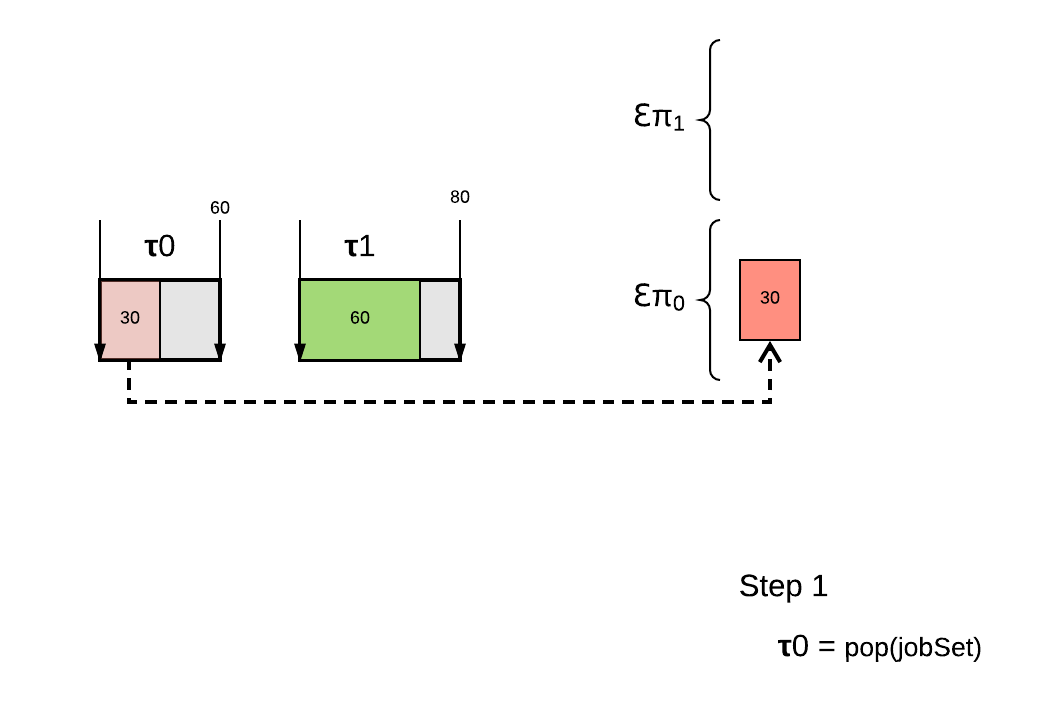
\includegraphics[scale=0.5]{img/gedf/gedf}
		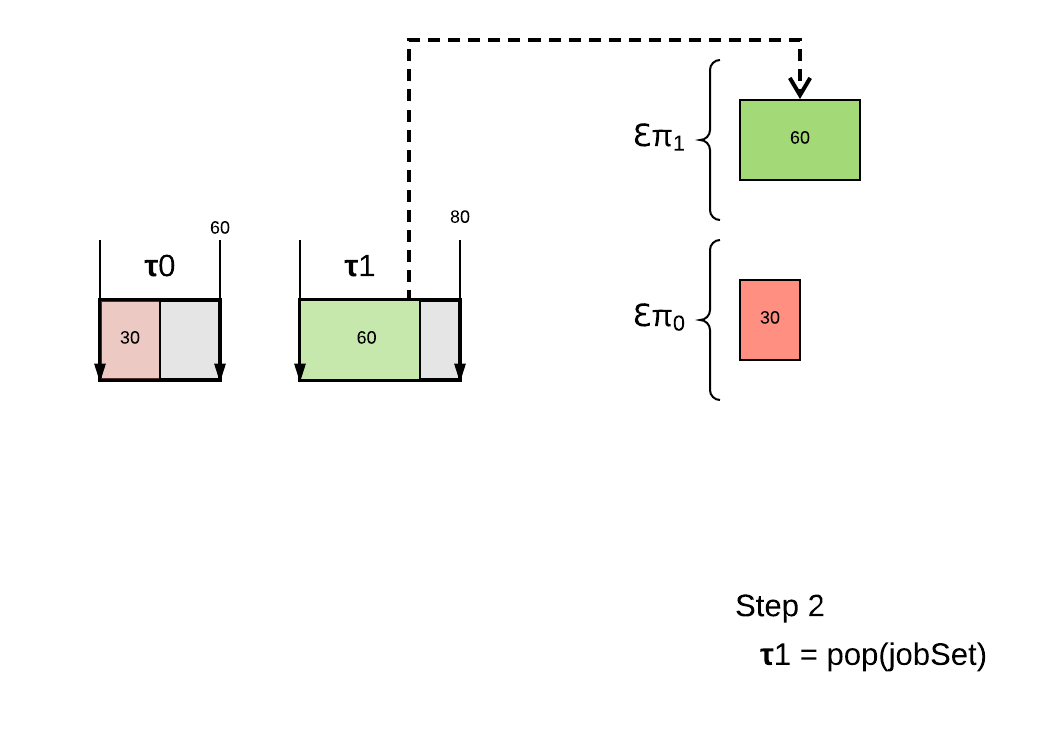
\includegraphics[scale=0.5]{img/gedf/gedf2}
		\caption{Global EDF}
	\end{figure}
	 
	On peut facilement voir que cela peut entraîner de \og{}mauvais choix\fg{}. 
	En changeant l'exemple précédent, et en prenant un exemple avec 3 travaux, 
	on n'obtiendra pas du tout le même ordonnancement dans les deux algorithmes, 
	et celui-ci mettra en échec \textbf{Global-EDF} quasiment immédiatement.\newline
	
	Prenons un ensemble de trois tâches comme suit :

	\begin{enumerate}
		\setlength\itemsep{0.1em}
		\item $\tau_1 : \{o:0; w:40; d=p:60;\}$
		\item $\tau_2 : \{o:0; w:40; d=p:60;\}$
		\item $\tau_3 : \{o:0; w:40; d=p:60;\}$
	\end{enumerate}
	
	\todo{insérer schema ici}
	
	Malgré ce point, \textbf{Global-EDF} est \og{}efficace\fg{} en terme de calculs.
	Le point le plus complexe concerne la structure de données qui conserve les 
	tâches courantes. Une bonne idée est d'utiliser un Heap [\ref*{heap}] qui 
	va permettre de fournir toujours en tête le travail de priorité supérieure.
	Pour s'assurer de la faisabilité de l'ensemble de tâches, 
	il faudra tester l'ordonnancement suffisamment longtemps (hyper-période).\newline

		
\section{HIPPEROS}
	\customhighlight{HIPPEROS} (\textbf{HI}gh \textbf{P}erformance \textbf{P}arallel \textbf{E}mbedded \textbf{R}eal-time \textbf{O}perating \textbf{S}ystems)
	est un \customhighlight{RTOS} (Real-Time Operating System) développé depuis plusieurs années par une spinoff de l'ULB.
	Il bénéficie des connaissances apportées par le monde de la recherche dans 
	le domaine des systèmes critiques avec multic\oe{}urs. Une de ses particularités 
	est sa modularité, qui permet d'adapter ses possibilités en fonction du système 
	lors de la compilation de l'OS, ainsi peut-on différencier principalement 
	deux installations en fonction des particularités. 
	
	\customhighlight{HIPPEROS} est un candidat idéal pour l'implémentation d'un ordonnanceur 
	global. Il a cependant un fonctionnement propre qui pourra rendre l'implémentation 
	plus ou moins facile. Par exemple, HIPPEROS, à l'inverse de \textit{Linux}, a un ordonnanceur 
	asymétrique (un processeur est \textit{Master}, et les autres sont \textit{Slaves}).
	En d'autres termes, l'ordonnancement est calculé uniquement sur l'un des processeurs, 
	qui sera désigné au moment de la compilation. 
	Cela simplifie l'implémentation, puisque l'on ne doit pas s'occuper de savoir quel processeur est 
	actuellement en train d'effectuer l'algorithme d'ordonnancement.\newline
	En résumé, une nouvelle implémentation sur un OS différent 
	peut elle-aussi apporter à la connaissance générale des détails importants.\newline
	
	Notons qu'HIPPEROS est un RTOS privé, avec les conséquences logistiques que l'on peut 
	imaginer : la documentation est privée également, et pour comprendre le kernel, la 
	seule ressource est l'équipe de développeurs qui l'a créé. 
	
		
\section{Attentes}

	Des présentations des différents acteurs qui ont été faites dans les parties précédentes, à savoir :
	\begin{enumerate}
		\setlength\itemsep{0.1em}
		\item UEDF
		\item Global-EDF
		\item HIPPEROS
	\end{enumerate}
	Nous pouvons déjà formuler certaines hypothèses que nous aimerions vérifier dans ce travail. \newline
	
	\begin{itemize}
		\item Vérifier que l'algorithme ne comporte rien qui empêche son implémentation dans 
		HIPPEROS
		\item Mesurer les surcoûts liés à l'algorithme \textbf{UEDF}, car il n'est pas 
		évident qu'il soit possible de l'utiliser en pratique.
		\item Vérifier également si l'on observe bien en pratique que \textbf{Global-EDF} ne 
		peut pas ordonnancer certains systèmes là où \textbf{UEDF} le peut.
		En effet, il est possible que ce résultat soit modifié ou largement à nuancer en 
		fonction de certains paramètres, comme le WCET, dont nous reparlerons.
		\item Comparer le nombre de migrations/préemptions obtenues pour un même système, ordonnancé 
		par l'un ou l'autre des algorithmes, on peut s'attendre à ce qu'\textbf{UEDF} soit performant à ce niveau.
	\end{itemize}

